\documentclass[10pt,conference,compsocconf]{IEEEtran}

\usepackage{hyperref}
\usepackage{hhline}
\usepackage{graphicx}	% For figure environment
\usepackage{amsmath, blkarray}


\begin{document}
\title{Machine Learning Project: Road Segmentation}

\author{Vincenzo Bazzucchi, Amaury Combes, Alexis Montavon}

\maketitle

\begin{abstract}
Road segmentation aims at distinguishing roads in satellite images.
It finds application in a multitude of domains such as map creation and updating, GPS technologies and traffic management. In this project we propose a technique to detect roads from satellite images using a convolutional neural network (CNN) trained on random batches to optimize running time and provide a good accuracy.
\end{abstract}

\section{Introduction}
The main task consists in classifying each pixel of an image to indicate whether it is a pixel of road (that we will indicate with class $1$) or not road (class $0$). Given the large number of pixels in images and the complex nature of the computations to perform, this problem was very complex to tackle. Today, thanks to the advent of multiprocessing, powerful Graphical Processing Units (GPUs) and advanced software libraries many possibilities can be considered. In this paper we expose our research through two models that we implemented and tested starting from a simple and interpretable one relying on a Multilayer Perceptron (MLP) to a more complex but accurate one using a CNN.\\
We will start by presenting both models and explain their general ideas, then go in more details about our implemtation. We will then described our results and discuss how it can be improved in a following study.

\section{Models}
Both our models rely on the same idea: classifying pixels independently only using their Red, Green and Blue (RGB) values does not perform well and does not make sense. We need to consider for each pixel, its \textbf{neighborhood}.

\subsection{The classical model: data matrix and multilayer perceptron}
This first method was strongly inspired by \cite{model1}.
The model takes, for each pixels, its RGB values and the values of the eight surrounding ones and flattens this 
27 values on a horizontal vector. The vertical stacking of all the vectors produces a matrix which has 27 features. The value is then fed to a multilayer perceptron: a neural network having three layers:
\begin{enumerate}
  \item a (fully connected) linear layer consisting of 27 neurons which uses the sigmoid function as the non-linear activation function: $$\sigma(x) = \frac{e^x}{1 + e^x}$$
  \item a hidden layer, another fully connected linear layer consisting, in the original paper, of 12 neurons using $\sigma$ as activation as well. We tried other values for the number of neurons.
\end{enumerate}

\begin{figure}[tp]
  \centering
  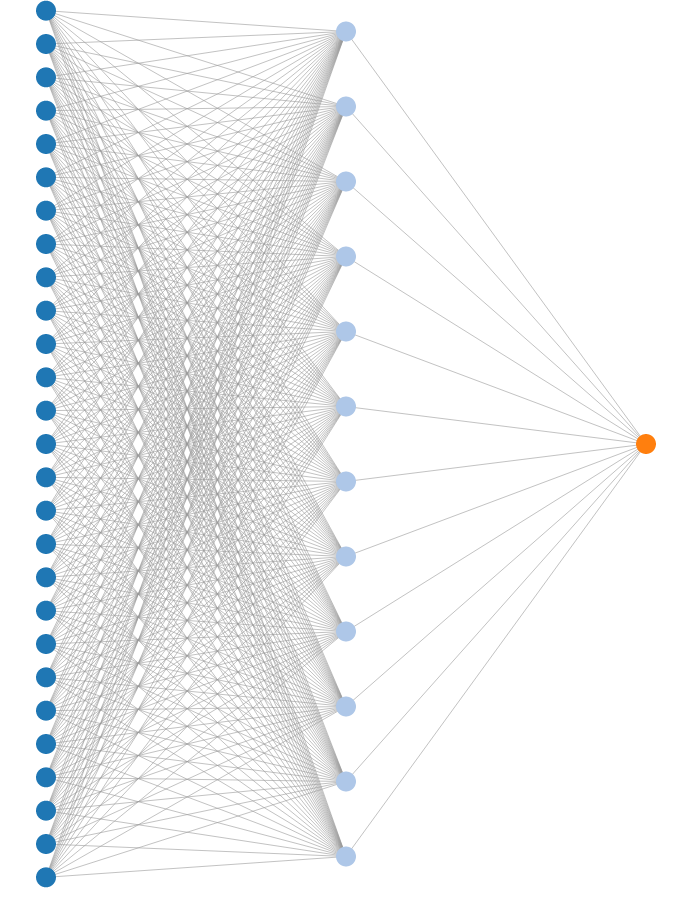
\includegraphics[height=0.6\columnwidth]{mlp-structure.png}
  \caption{Structure of the Multilayer Perceptron used in Model A, the input neurons are in blue and the output neuron is orange}
  \vspace{-3mm}
  \label{fig:mlp-structure}
\end{figure}

The structure of the neural net is shown in Figure \ref{fig:mlp-structure}
We used a learning rate of $0.01$.

\subsection{The more complex model: using a convolutional neural network}
As we will discuss in the results \ref{results} section, the results of the previous method lead us to look for alternatives.
We decided to try a convolutional neural network to classify each pixel, using its neighborhood. The idea of distinguishing whether the center of a square of pixels was road or not looked to us very similar to the problem of image classification. Therefore we built a CNN with a structure very close to the one used for this purpose. For the structure of the NN, we implemented a simplified version of the one proposed here\cite{stanford}: instead of the complex model \texttt{INPUT -> [[CONV -> RELU]*N -> POOL?]*M -> [FC -> RELU]*K -> FC} we used 4 [\texttt{CONV, RELU, MAX}] followed by two linear layers. For the output dimensions of the convolutions, we learned in class that usually they reduce the width and height of the image (valid padding) and that the output channels or depth increases at each layer.

However as convolutions rely on the structure of the images that they manipulate, we had to change our preprocessing: instead of creating, for each pixel and its neighborhood, a line for a matrix, we create a tensor having dimensions the width and height of the neighborhood and the number of channels (3 for RGB). All the tensors are stacked and fed to the CNN.
The CNN has the structure depicted in the following table:

\begin{center}
\begin{tabular}{c | c | c}
Input shape & Type of layer & Output shape \\ \hhline{===}
$(b, 71, 71, 3)$ & 2D Convolution size 5 & $(b, 67, 67, 32)$ \\
$(b, 67, 67, 32)$ & Leaky ReLU Activation & $(b, 67, 67, 32)$ \\
$(b, 67, 67, 32)$ & 2D Max Pooling & $(b, 33, 33, 32)$ \\ \hline

$(b, 33, 33, 32)$ & 2D Convolution size 3 & $(b, 31, 31, 64)$ \\
$(b, 31, 31, 64)$ & Leaky ReLU Activation  & $(b, 31, 31, 64)$ \\
$(b, 31, 31, 64)$ & 2D Max Pooling & $(b, 15, 15, 64)$ \\ \hline

$(b, 15, 15, 64)$ & 2D Convolution size 3 & $(b, 13, 13, 128)$ \\
$(b, 13, 13, 128)$ & Leaky ReLU Activation  & $(b, 13, 13, 128)$ \\
$(b, 13, 13, 128)$ & 2D Max Pooling & $(b, 6, 6, 128)$ \\ \hline

$(b, 6, 6, 128)$ & 2D Convolution size 3 & $(b, 4, 4, 256)$ \\
$(b, 4, 4, 256)$ & Leaky ReLU Activation  & $(b, 4, 4, 256)$ \\
$(b, 4, 4, 256)$ & 2D Max Pooling & $(b, 2, 2, 256)$ \\ \hline

$(b, 2, 2, 256)$ & Fully Connected Linear & $(b, 2, 2, 128)$ \\
$(b, 2, 2, 128)$ & Leaky ReLU Activation  & $(b, 2, 2, 128)$ \\ \hline

$(b, 2, 2, 128 )$ & Reshape & $(b, 512)$ \\ \hline
$(b, 512)$ & Fully Connected Linear & $(b, 2)$ \\
$(b, 2)$ & Sigmoid Activation & $(b, 2)$
\end{tabular}
\end{center}

All the convolutions have \textbf{stride $1$} to be sure to classify all pixels.
$b$ is the batch size, the number of neighborhoods fed into the CNN at each epoch and its choice is discussed in \ref{perf}.
Between every convolutional layer we use dropout with probability $1/4$ to avoid overfitting.
The first four convolutional layers are used to learn some characteristics of the neighborhood that the CNN is
analyzing while the two final fully connected layers act as a classifier.

\section{Implementation}
All our code is written in the Python programming language using the following libraries:
\begin{itemize}
\item numpy for array and tensor manipulation
\item skimage and scipy for image processing (such as RGB to HSV conversion)
\item matplotlib for exploratory plots and for loading images
\item Keras \cite{chollet2015keras} as our Machine Learning framework using the TensorFlow backend.
\end{itemize}

\subsection{General Preprocessing}
For the image preprocessing, we decided to switch our pixels from the RGB colorspace to the HSV colorspace. As we can see below, the HSV colorspace yields much more indepedent (smaller correlation) features compared to the RGB colorspace.  

$$
    \bordermatrix{ & h & s & v \cr
      h & 1. & 0.13011035 & -0.10973323 \cr
      s & 0.13011035 & 1. & -0.47243836 \cr
      v & -0.10973323 & -0.47243836 & 1. } \qquad
$$

\begin{center}
HSV correlation matrix
\end{center}
$$
     \bordermatrix{ & r & g & b \cr
      r & 1. & 0.98716897 & 0.98023219 \cr
      g & 0.98716897 & 1. & 0.98806847 \cr
      b & 0.98023219 & 0.98806847 & 1. } \qquad
$$

\begin{center}
RGB correlation matrix
\end{center}

\subsection{Neighborhood cropping}
\subsubsection{Boundary conditions}
In both of our models, we take for each pixel, its RGB values and the RGB values of a number $N$ of surrounding pixels.
We defined a neighborhood as \textbf{squared region} of the image having odd dimension.
The problem of boundary regions arises: what pixel values should we take as neighbors for the pixels on the edges of the image? We decided to pad the image with the minimal number of pixels so that every pixel that we need to classify has a the required number of neighbors. As zero padding would have added potentially confusing information for our models, we padded our images by mirroring their edges. For example, if the neighborhood size is $37$, we pad the image with a border of width $18 = (37 - 1)/2$. An example can be found in Figure \ref{fig:padding-example}: here we added a mirrored padding of size 40. The blue color is only to highlight the region for explanatory purpose and is not present in the images fed to our models.\\ The code responsible for padding is implemented in the function \texttt{reflect-padding} in \texttt{preprocessing.py}

\begin{figure}[h]
  \centering
  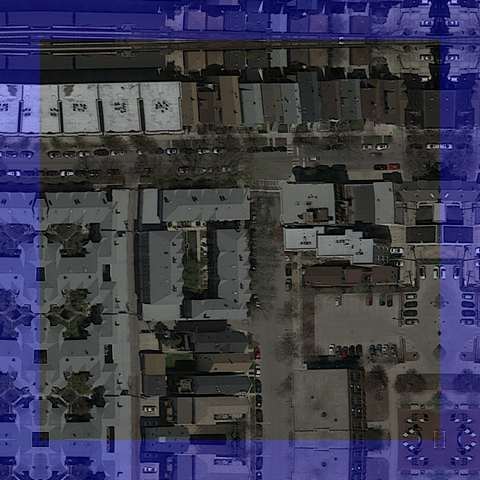
\includegraphics[width=0.6\columnwidth]{padding_example-borderwidth40.png}
  \caption{Mirroring padding example: padding width 40}
  \vspace{-3mm}
  \label{fig:padding-example}
\end{figure}

\subsubsection{Neighborhood extraction}
As mentioned earlier, for each pixel we extract the squared patch centered around that pixel. To extract all neighborhood we iterate over all pixels one by one and for each one we use numpy's slicing functionalities to select the region. This is implemented in the function \texttt{neighborhood-iter} in \texttt{preprocessing.py}. The \texttt{image\_to\_features} and \texttt{image\_to\_neighborhoods} extract all neighbors for the given image returning a matrix for the first one and a tensor for the second one.

\subsubsection{Weight and bias initializations}
For both models we use Xavier\cite{xavier-init} initialization to initialize the weights of the neural networks while the biases are initialized to zero.

\subsection{Model A}
The preprocessing of this model is illustrated in Figure \ref{fig:mlp-preproc}. The reasons and implementation of patching are discussed in \ref{perf}. 
The implementation of this model is done using Keras' \texttt{sequential} to compose the two linear models and associated sigmoid activations.
We use the built-in Adam optimizer to reduce the mean squared error.

\begin{figure}[t]
  \centering
  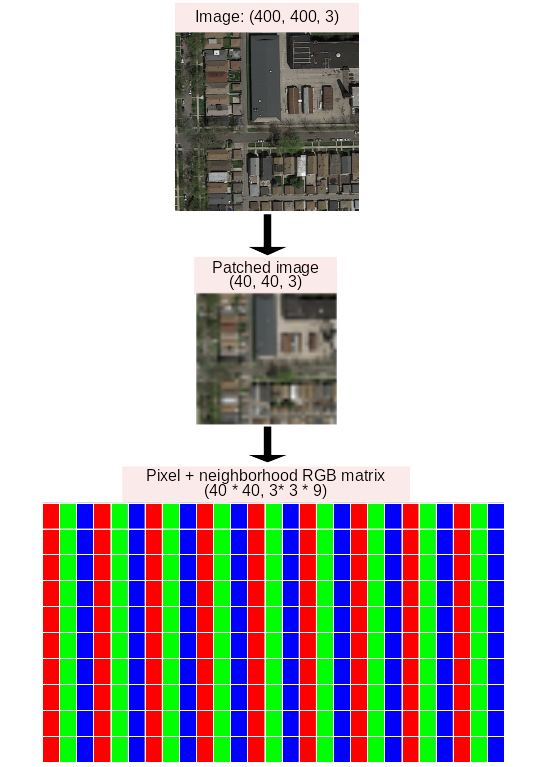
\includegraphics[height=0.7\columnwidth]{mlp-preprocessing-schema.png}
  \caption{Preprocessing pipeline for Model A.}
  \vspace{-3mm}
  \label{fig:mlp-preproc}
\end{figure}

\subsection{Model B}
The preprocessing of this model is illustrated in Figure \ref{fig:cnn-preproc}
The implementation of this model is done using Keras' \texttt{sequential} to compose the layers. All the layers' implementations are defined in the library. We used the Adam optimizer and the Categorical Cross Entropy loss function.
The categorical cross entropy loss function is one of the most used loss functions for classifications problems. In order to use it we had to transform the labels obtained by the ground truth images: instead of a single floating point value per pixel we first generated an indicator with value $1$ if the pixel is road and $0$ otherwise.
We then transformed each of this value in a tuple the first value of which is one if the pixel is not road and the second one is $1$ if the pixel is road.\\
The learning rate used is $0.001$.\\
When dealing with CNN, the Rectified Linear Unit (ReLU) is one of the most used activation functions but it exposes the model to the risk of \textit{dead filters} \cite{leakyrelu}. In the same paper we learn that to avoid the null gradients caused by the standard ReLU, when this returns 0, we replace it with a small $\alpha < 1$ of $0.1$.
Finally we used erosion and dilation methods to remove the noise on the predicted images and improve our score a little more. We used the \texttt{opening} and \texttt{closing} methods from skimage.

\begin{figure}[t]
  \centering
  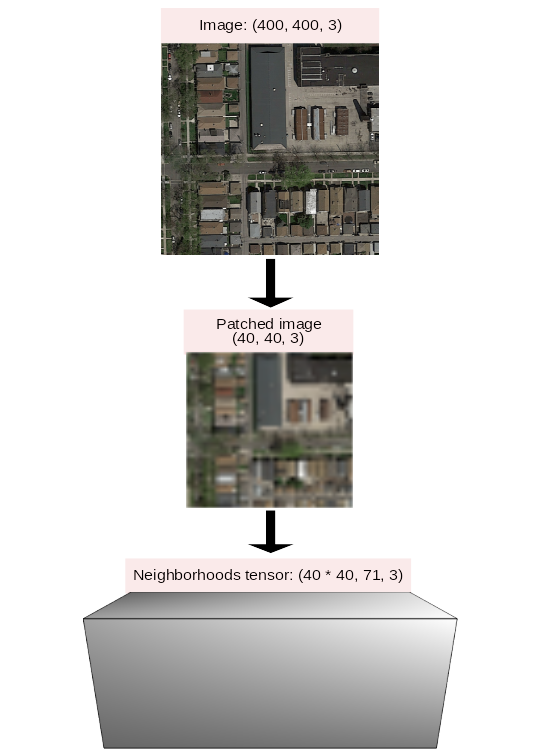
\includegraphics[height=0.7\columnwidth]{cnn-preprocessing-schema.png}
  \caption{Preprocessing pipeline for Model B.}
  \vspace{-3mm}
  \label{fig:cnn-preproc}
\end{figure}

\subsection{Improving performances} \label{perf}
The training sets consists of $100$ $400\times400$ images. When they are loaded into memory, each RGB component of each pixel is stored in a 32-bit floating point variable. Thus $100\times3\times 400² = 4.8 \cdot 10^7$ variables are allocated on memory. When the neighborhoods are extracted, the size of the dataset grows: for each pixel, we have to consider its neighbors. For instance in our second model, each neighborhood has size $71\times71$ which means that the number of 32 bit floating point values grows to $3 \times 100 \times 400^2 \times 71^2 = 2.41968 \cdot 10^{11}$. Even without considering the groundtruths images, it becomes challenging for common machines to have such amounts of RAM to perform computations.
We therefore implemented two techniques to reduce the memory impact and to improve computation times.

\subsubsection{Patching}
The size of the image is reduced by taking, for a squared region of size $P\times P$, the average of the values of each of component (R, G and B) of the pixels in the image. The compromise between quality and compression that we found is to use $P=10$. An illustration can be found in Figure \ref{fig:patching}.
To be able to associate each patch to a label (road/not road) we had to apply the same treatment to the groundtruth images. However each patch needs to be either 1 or 0 and not some value in the range between the two. Therefore for each patch of the groundtruth we sum up all the values of the pixels in it and if 25\% or more pixels of the patch have label 1, then the patch has label $1$ otherwise it has label $0$.\\
This is implemented in the functions \texttt{patch\_image} and \texttt{patch\_groundtruth} which rely on \texttt{patch\_map} in the \texttt{preprocessing.py} file. The \texttt{unpatch} function was defined to enlarge compressed images back to the original format.\\
The use of patching and of the mirroring done in neighborhood extraction allowed us to consider for each pixel, not only the neighbor pixels, but the entire image centered at that pixel. In other words to classify each pixel, we look at the entire picture, much alike to what the human eye would do.
\begin{figure}[h]
  \centering
  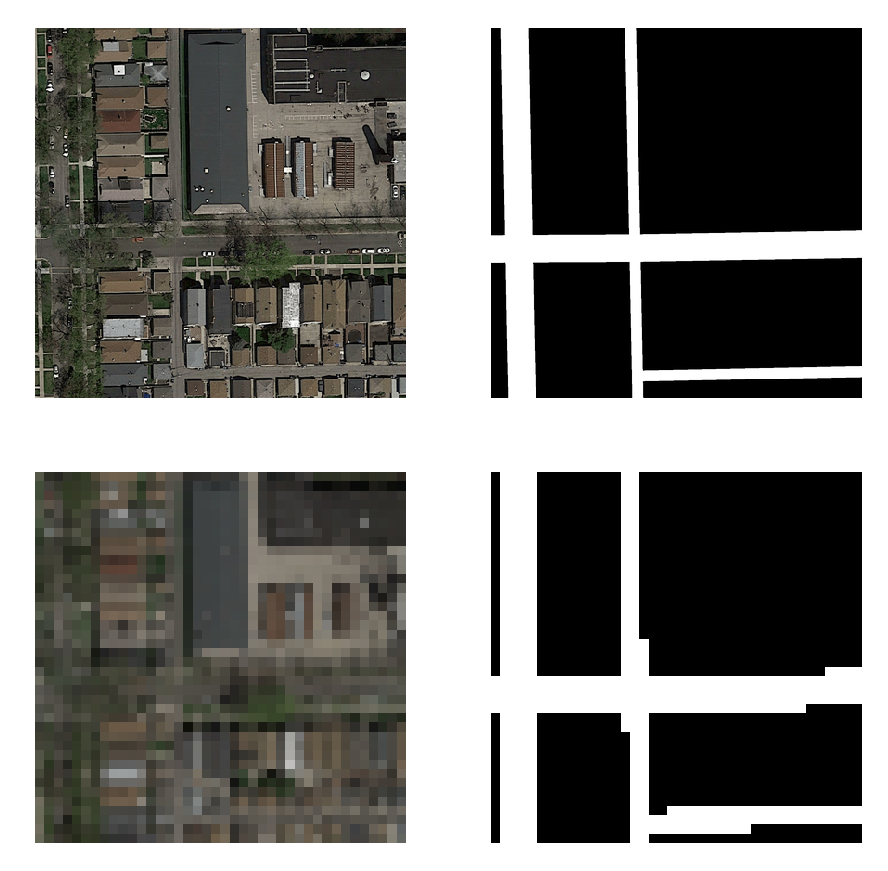
\includegraphics[height=0.6\columnwidth]{patching.png}
  \caption{The first rows shows one of the images and the associated groundtruth. The second one shows the same images compressed using patching with $P=10$}
  \vspace{-3mm}
  \label{fig:patching}
\end{figure}


\subsubsection{Batching}
Even by reducing the size of the images and therefore the number of neighborhoods used for training using the previous technique, the whole tensor of neighborhoods does not fit into memory. If a subset of the training images is used, we can fit all the neighborhoods into memory, but each epoch runs very slowly. Therefore, instead of feeding all the neighborhoods at each epoch, only $b$ of them are randomly chosen and used at any given epoch. This feature is provided out of the box by Keras using the \texttt{batch\_size} argument of the \texttt{fit} method of the \texttt{Model} class. The value used to produced our best score was \textbf{1600}.

\section{Results} \label{results}
\subsection{Model A}
We ran the implementation proposed in \cite{model1} varying the neighborhood size and the number of neurons in the hidden layer of the MLP. The resulting F1 scores are reported in the heatmap in Figure\ref{fig:heatmap}
\begin{figure}[h]
  \centering
  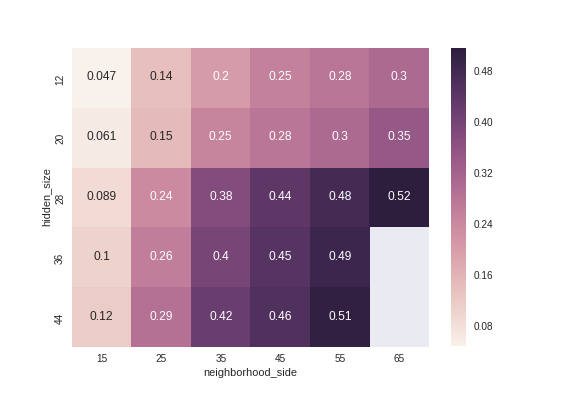
\includegraphics[width=\columnwidth]{mlp_gridsearch.png}
  \caption{F1 scores obtained with 3-folds cross validation during the gridsearch for the hidden size and neighborhood size of the MLP}
  \vspace{-3mm}
  \label{fig:heatmap}
\end{figure}

\subsection{Model B}
As a true cross validation on this model is not feasible with our computational resources, to test multiples hyper-parameters we trained on 70\% of our training set and tested on the remaining. We started by comparing different number of epochs the results are given in the table below. And from there we chose to keep \textbf{100} epochs for our best model.
\begin{center}
\begin{tabular}{c | c}
\#Epochs & F1 score\\ \hhline{==}
$25$ & $0.80487$\\
$50$ & $0.80560$\\
$100$ & $0.80596$\\
$200$ & $0.80547$
\end{tabular}
\end{center}

We then turned our attention to the size of the neighborhood to feed the neural network. Understand that the smaller this size is, the less information is given to model about the adjacent pixels. We ran our model with a small window of 41x41 and obtained a score of $0.66722\%$ we then augmented this size until reached a better one, keeping in mind that the bigger the size is, the more padding we must add. A good compromise was found using a window size of \textbf{71}. The model run with all these parameters on the full training set gave us a score of \textbf{0.86038} on Kaggle.
Fig. \ref{overlay} shows the first test image with our prediction.

\begin{figure}[h]
  \centering
  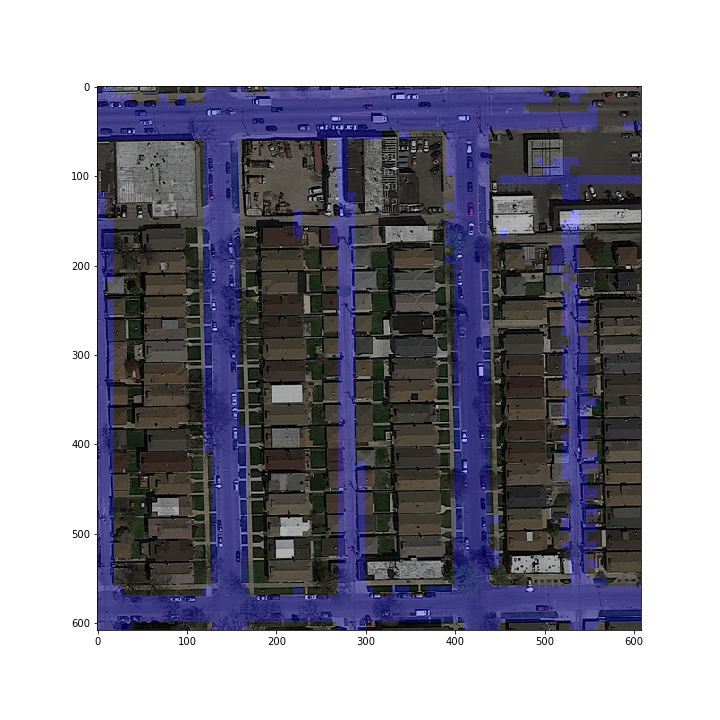
\includegraphics[width=\columnwidth]{overlay_rapport.png}
  \caption{Prediction on the first test image}
  \vspace{-3mm}
  \label{overlay}
\end{figure}


\section{Conclusion} \label{conclusion}
As already discussed, road segmentation is a well known exercise and a lot of research have already been conducted. We followed an accurate and complicated system done in \cite{stanford} and modified it to fit our vision and computational resources while keeping a pretty descent score. As it can be seen in Fig. \ref{overlay} the predictions are not perfect but the model still performs well. It would be interesting to take it some step further and try to make this model more complex.
\bibliographystyle{IEEEtran}
\bibliography{literature}

\end{document}
